\begin{figure*}
\definecolor{R}{rgb}{1,0,0} % red
\definecolor{G}{rgb}{0,0.6,0.36078431372} % forestgreen
\definecolor{B}{rgb}{0,0,1} % blue
\definecolor{O}{rgb}{0.99607843137,0.63529411764,0.22745098039} % orange
\definecolor{P}{rgb}{0.60784313725,0.27843137254,0.58823529411} % purple
\centering
% \newcommand{\uniquesize}{0.13\textwidth}
\newcommand{\uniquesize}{0.157\textwidth}
%
%
%
\begin{subfigure}[b]{\uniquesize}
\centering
\resizebox{!}{\textwidth}{
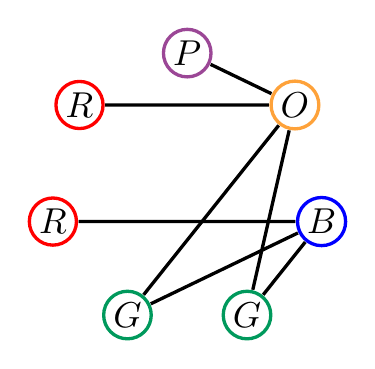
\begin{tikzpicture}[
mynode/.style={draw, circle, very thick, inner sep=1pt, scale=1.3},
myline/.style={draw, very thick},
]
\pgfmathsetmacro{\n}{7};
\pgfmathsetmacro{\r}{1.75};
\node[mynode,draw=P] (1) at (0*360/\n + 90: \r cm) {$\xcolor{P}$};
\node[mynode,draw=R] (2) at (1*360/\n + 90: \r cm) {$\xcolor{R}$};
\node[mynode,draw=R] (3) at (2*360/\n + 90: \r cm) {$\xcolor{R}$};
\node[mynode,draw=G] (4) at (3*360/\n + 90: \r cm) {$\xcolor{G}$};
\node[mynode,draw=G] (5) at (4*360/\n + 90: \r cm) {$\xcolor{G}$};
\node[mynode,draw=B] (6) at (5*360/\n + 90: \r cm) {$\xcolor{B}$};
\node[mynode,draw=O] (7) at (6*360/\n + 90: \r cm) {$\xcolor{O}$};
\draw [myline] (7) -- (1);
\draw [myline] (7) -- (2);
\draw [myline] (6) -- (3);
\draw [myline] (6) -- (4);
\draw [myline] (7) -- (4);
\draw [myline] (6) -- (5);
\draw [myline] (7) -- (5);
\end{tikzpicture}
}
\caption{\mypm{}~54923}
\end{subfigure}
%
%
%
\begin{subfigure}[b]{\uniquesize}
\centering
\resizebox{!}{\textwidth}{
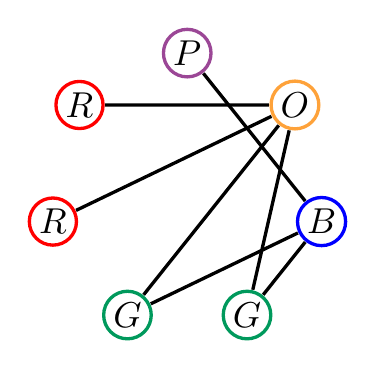
\begin{tikzpicture}[
mynode/.style={draw, circle, very thick, inner sep=1pt, scale=1.3},
myline/.style={draw, very thick},
]
\pgfmathsetmacro{\n}{7};
\pgfmathsetmacro{\r}{1.75};
\node[mynode,draw=P] (1) at (0*360/\n + 90: \r cm) {$\xcolor{P}$};
\node[mynode,draw=R] (2) at (1*360/\n + 90: \r cm) {$\xcolor{R}$};
\node[mynode,draw=R] (3) at (2*360/\n + 90: \r cm) {$\xcolor{R}$};
\node[mynode,draw=G] (4) at (3*360/\n + 90: \r cm) {$\xcolor{G}$};
\node[mynode,draw=G] (5) at (4*360/\n + 90: \r cm) {$\xcolor{G}$};
\node[mynode,draw=B] (6) at (5*360/\n + 90: \r cm) {$\xcolor{B}$};
\node[mynode,draw=O] (7) at (6*360/\n + 90: \r cm) {$\xcolor{O}$};
\draw [myline] (6) -- (1);
\draw [myline] (7) -- (2);
\draw [myline] (7) -- (3);
\draw [myline] (6) -- (4);
\draw [myline] (7) -- (4);
\draw [myline] (6) -- (5);
\draw [myline] (7) -- (5);
\end{tikzpicture}
}
\caption{\mypm{}~55043}
\end{subfigure}
%
%
%
\begin{subfigure}[b]{\uniquesize}
\centering
\resizebox{!}{\textwidth}{
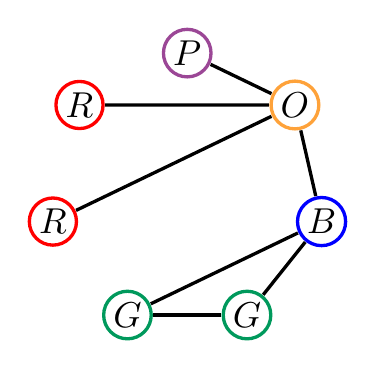
\begin{tikzpicture}[
mynode/.style={draw, circle, very thick, inner sep=1pt, scale=1.3},
myline/.style={draw, very thick},
]
\pgfmathsetmacro{\n}{7};
\pgfmathsetmacro{\r}{1.75};
\node[mynode,draw=P] (1) at (0*360/\n + 90: \r cm) {$\xcolor{P}$};
\node[mynode,draw=R] (2) at (1*360/\n + 90: \r cm) {$\xcolor{R}$};
\node[mynode,draw=R] (3) at (2*360/\n + 90: \r cm) {$\xcolor{R}$};
\node[mynode,draw=G] (4) at (3*360/\n + 90: \r cm) {$\xcolor{G}$};
\node[mynode,draw=G] (5) at (4*360/\n + 90: \r cm) {$\xcolor{G}$};
\node[mynode,draw=B] (6) at (5*360/\n + 90: \r cm) {$\xcolor{B}$};
\node[mynode,draw=O] (7) at (6*360/\n + 90: \r cm) {$\xcolor{O}$};
\draw [myline] (7) -- (1);
\draw [myline] (7) -- (2);
\draw [myline] (7) -- (3);
\draw [myline] (5) -- (4);
\draw [myline] (6) -- (4);
\draw [myline] (6) -- (5);
\draw [myline] (7) -- (6);
\end{tikzpicture}
}
\caption{\mypm{}~95560}
\end{subfigure}
%
%
%
\begin{subfigure}[b]{\uniquesize}
\centering
\resizebox{!}{\textwidth}{
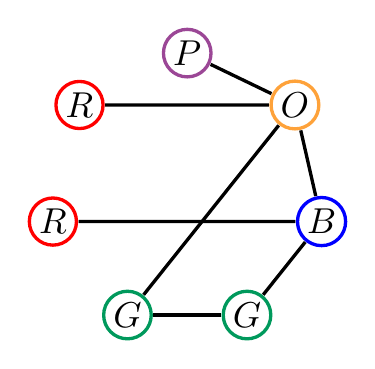
\begin{tikzpicture}[
mynode/.style={draw, circle, very thick, inner sep=1pt, scale=1.3},
myline/.style={draw, very thick},
]
\pgfmathsetmacro{\n}{7};
\pgfmathsetmacro{\r}{1.75};
\node[mynode,draw=P] (1) at (0*360/\n + 90: \r cm) {$\xcolor{P}$};
\node[mynode,draw=R] (2) at (1*360/\n + 90: \r cm) {$\xcolor{R}$};
\node[mynode,draw=R] (3) at (2*360/\n + 90: \r cm) {$\xcolor{R}$};
\node[mynode,draw=G] (4) at (3*360/\n + 90: \r cm) {$\xcolor{G}$};
\node[mynode,draw=G] (5) at (4*360/\n + 90: \r cm) {$\xcolor{G}$};
\node[mynode,draw=B] (6) at (5*360/\n + 90: \r cm) {$\xcolor{B}$};
\node[mynode,draw=O] (7) at (6*360/\n + 90: \r cm) {$\xcolor{O}$};
\draw [myline] (7) -- (1);
\draw [myline] (7) -- (2);
\draw [myline] (6) -- (3);
\draw [myline] (5) -- (4);
\draw [myline] (7) -- (4);
\draw [myline] (6) -- (5);
\draw [myline] (7) -- (6);
\end{tikzpicture}
}
\caption{\mypm{}~96505}
\end{subfigure}
%
%
%
\begin{subfigure}[b]{\uniquesize}
\centering
\resizebox{!}{\textwidth}{
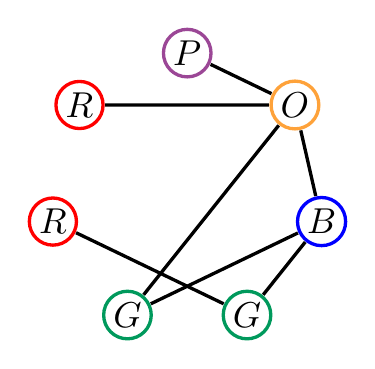
\begin{tikzpicture}[
mynode/.style={draw, circle, very thick, inner sep=1pt, scale=1.3},
myline/.style={draw, very thick},
]
\pgfmathsetmacro{\n}{7};
\pgfmathsetmacro{\r}{1.75};
\node[mynode,draw=P] (1) at (0*360/\n + 90: \r cm) {$\xcolor{P}$};
\node[mynode,draw=R] (2) at (1*360/\n + 90: \r cm) {$\xcolor{R}$};
\node[mynode,draw=R] (3) at (2*360/\n + 90: \r cm) {$\xcolor{R}$};
\node[mynode,draw=G] (4) at (3*360/\n + 90: \r cm) {$\xcolor{G}$};
\node[mynode,draw=G] (5) at (4*360/\n + 90: \r cm) {$\xcolor{G}$};
\node[mynode,draw=B] (6) at (5*360/\n + 90: \r cm) {$\xcolor{B}$};
\node[mynode,draw=O] (7) at (6*360/\n + 90: \r cm) {$\xcolor{O}$};
\draw [myline] (7) -- (1);
\draw [myline] (7) -- (2);
\draw [myline] (5) -- (3);
\draw [myline] (6) -- (4);
\draw [myline] (7) -- (4);
\draw [myline] (6) -- (5);
\draw [myline] (7) -- (6);
\end{tikzpicture}
}
\caption{\mypm{}~96506}
\end{subfigure}
%
%
%
\begin{subfigure}[b]{\uniquesize}
\centering
\resizebox{!}{\textwidth}{
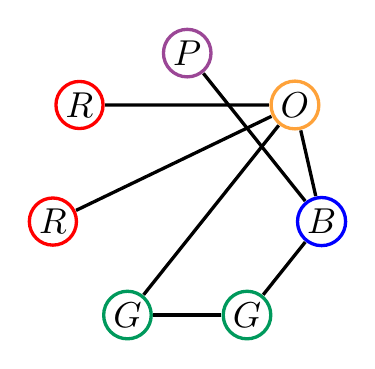
\begin{tikzpicture}[
mynode/.style={draw, circle, very thick, inner sep=1pt, scale=1.3},
myline/.style={draw, very thick},
]
\pgfmathsetmacro{\n}{7};
\pgfmathsetmacro{\r}{1.75};
\node[mynode,draw=P] (1) at (0*360/\n + 90: \r cm) {$\xcolor{P}$};
\node[mynode,draw=R] (2) at (1*360/\n + 90: \r cm) {$\xcolor{R}$};
\node[mynode,draw=R] (3) at (2*360/\n + 90: \r cm) {$\xcolor{R}$};
\node[mynode,draw=G] (4) at (3*360/\n + 90: \r cm) {$\xcolor{G}$};
\node[mynode,draw=G] (5) at (4*360/\n + 90: \r cm) {$\xcolor{G}$};
\node[mynode,draw=B] (6) at (5*360/\n + 90: \r cm) {$\xcolor{B}$};
\node[mynode,draw=O] (7) at (6*360/\n + 90: \r cm) {$\xcolor{O}$};
\draw [myline] (6) -- (1);
\draw [myline] (7) -- (2);
\draw [myline] (7) -- (3);
\draw [myline] (5) -- (4);
\draw [myline] (7) -- (4);
\draw [myline] (6) -- (5);
\draw [myline] (7) -- (6);
\end{tikzpicture}
}
\caption{\mypm{}~96625}
\end{subfigure}
%
%
%

\begin{subfigure}[b]{\uniquesize}
\centering
\resizebox{!}{\textwidth}{
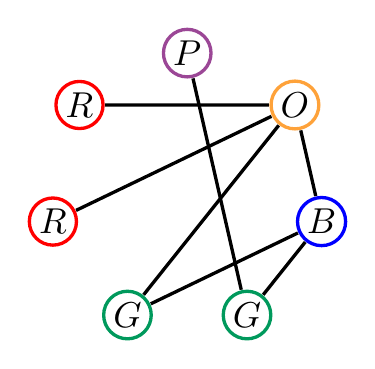
\begin{tikzpicture}[
mynode/.style={draw, circle, very thick, inner sep=1pt, scale=1.3},
myline/.style={draw, very thick},
]
\pgfmathsetmacro{\n}{7};
\pgfmathsetmacro{\r}{1.75};
\node[mynode,draw=P] (1) at (0*360/\n + 90: \r cm) {$\xcolor{P}$};
\node[mynode,draw=R] (2) at (1*360/\n + 90: \r cm) {$\xcolor{R}$};
\node[mynode,draw=R] (3) at (2*360/\n + 90: \r cm) {$\xcolor{R}$};
\node[mynode,draw=G] (4) at (3*360/\n + 90: \r cm) {$\xcolor{G}$};
\node[mynode,draw=G] (5) at (4*360/\n + 90: \r cm) {$\xcolor{G}$};
\node[mynode,draw=B] (6) at (5*360/\n + 90: \r cm) {$\xcolor{B}$};
\node[mynode,draw=O] (7) at (6*360/\n + 90: \r cm) {$\xcolor{O}$};
\draw [myline] (5) -- (1);
\draw [myline] (7) -- (2);
\draw [myline] (7) -- (3);
\draw [myline] (6) -- (4);
\draw [myline] (7) -- (4);
\draw [myline] (6) -- (5);
\draw [myline] (7) -- (6);
\end{tikzpicture}
}
\caption{\mypm{}~96626}
\end{subfigure}
%
%
%
\begin{subfigure}[b]{\uniquesize}
\centering
\resizebox{!}{\textwidth}{
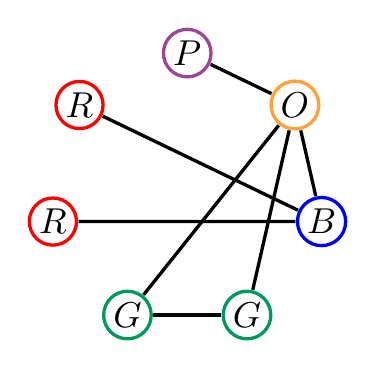
\begin{tikzpicture}[
mynode/.style={draw, circle, very thick, inner sep=1pt, scale=1.3},
myline/.style={draw, very thick},
]
\pgfmathsetmacro{\n}{7};
\pgfmathsetmacro{\r}{1.75};
\node[mynode,draw=P] (1) at (0*360/\n + 90: \r cm) {$\xcolor{P}$};
\node[mynode,draw=R] (2) at (1*360/\n + 90: \r cm) {$\xcolor{R}$};
\node[mynode,draw=R] (3) at (2*360/\n + 90: \r cm) {$\xcolor{R}$};
\node[mynode,draw=G] (4) at (3*360/\n + 90: \r cm) {$\xcolor{G}$};
\node[mynode,draw=G] (5) at (4*360/\n + 90: \r cm) {$\xcolor{G}$};
\node[mynode,draw=B] (6) at (5*360/\n + 90: \r cm) {$\xcolor{B}$};
\node[mynode,draw=O] (7) at (6*360/\n + 90: \r cm) {$\xcolor{O}$};
\draw [myline] (7) -- (1);
\draw [myline] (6) -- (2);
\draw [myline] (6) -- (3);
\draw [myline] (5) -- (4);
\draw [myline] (7) -- (4);
\draw [myline] (7) -- (5);
\draw [myline] (7) -- (6);
\end{tikzpicture}
}
\caption{\mypm{}~99544}
\end{subfigure}
%
%
%
\begin{subfigure}[b]{\uniquesize}
\centering
\resizebox{!}{\textwidth}{
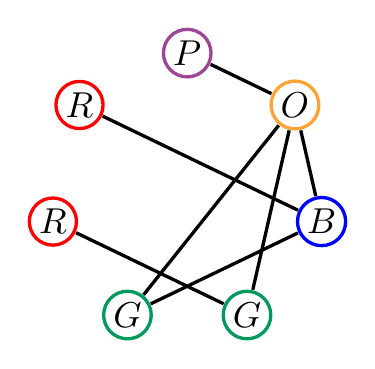
\begin{tikzpicture}[
mynode/.style={draw, circle, very thick, inner sep=1pt, scale=1.3},
myline/.style={draw, very thick},
]
\pgfmathsetmacro{\n}{7};
\pgfmathsetmacro{\r}{1.75};
\node[mynode,draw=P] (1) at (0*360/\n + 90: \r cm) {$\xcolor{P}$};
\node[mynode,draw=R] (2) at (1*360/\n + 90: \r cm) {$\xcolor{R}$};
\node[mynode,draw=R] (3) at (2*360/\n + 90: \r cm) {$\xcolor{R}$};
\node[mynode,draw=G] (4) at (3*360/\n + 90: \r cm) {$\xcolor{G}$};
\node[mynode,draw=G] (5) at (4*360/\n + 90: \r cm) {$\xcolor{G}$};
\node[mynode,draw=B] (6) at (5*360/\n + 90: \r cm) {$\xcolor{B}$};
\node[mynode,draw=O] (7) at (6*360/\n + 90: \r cm) {$\xcolor{O}$};
\draw [myline] (7) -- (1);
\draw [myline] (6) -- (2);
\draw [myline] (5) -- (3);
\draw [myline] (6) -- (4);
\draw [myline] (7) -- (4);
\draw [myline] (7) -- (5);
\draw [myline] (7) -- (6);
\end{tikzpicture}
}
\caption{\mypm{}~99547}
\end{subfigure}
%
%
%
\begin{subfigure}[b]{\uniquesize}
\centering
\resizebox{!}{\textwidth}{
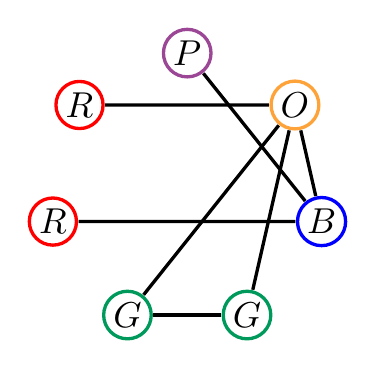
\begin{tikzpicture}[
mynode/.style={draw, circle, very thick, inner sep=1pt, scale=1.3},
myline/.style={draw, very thick},
]
\pgfmathsetmacro{\n}{7};
\pgfmathsetmacro{\r}{1.75};
\node[mynode,draw=P] (1) at (0*360/\n + 90: \r cm) {$\xcolor{P}$};
\node[mynode,draw=R] (2) at (1*360/\n + 90: \r cm) {$\xcolor{R}$};
\node[mynode,draw=R] (3) at (2*360/\n + 90: \r cm) {$\xcolor{R}$};
\node[mynode,draw=G] (4) at (3*360/\n + 90: \r cm) {$\xcolor{G}$};
\node[mynode,draw=G] (5) at (4*360/\n + 90: \r cm) {$\xcolor{G}$};
\node[mynode,draw=B] (6) at (5*360/\n + 90: \r cm) {$\xcolor{B}$};
\node[mynode,draw=O] (7) at (6*360/\n + 90: \r cm) {$\xcolor{O}$};
\draw [myline] (6) -- (1);
\draw [myline] (7) -- (2);
\draw [myline] (6) -- (3);
\draw [myline] (5) -- (4);
\draw [myline] (7) -- (4);
\draw [myline] (7) -- (5);
\draw [myline] (7) -- (6);
\end{tikzpicture}
}
\caption{\mypm{}~99559}
\end{subfigure}
%
%
%
\begin{subfigure}[b]{\uniquesize}
\centering
\resizebox{!}{\textwidth}{
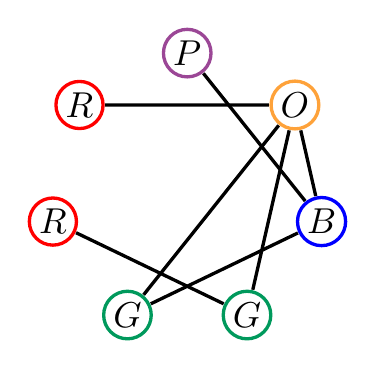
\begin{tikzpicture}[
mynode/.style={draw, circle, very thick, inner sep=1pt, scale=1.3},
myline/.style={draw, very thick},
]
\pgfmathsetmacro{\n}{7};
\pgfmathsetmacro{\r}{1.75};
\node[mynode,draw=P] (1) at (0*360/\n + 90: \r cm) {$\xcolor{P}$};
\node[mynode,draw=R] (2) at (1*360/\n + 90: \r cm) {$\xcolor{R}$};
\node[mynode,draw=R] (3) at (2*360/\n + 90: \r cm) {$\xcolor{R}$};
\node[mynode,draw=G] (4) at (3*360/\n + 90: \r cm) {$\xcolor{G}$};
\node[mynode,draw=G] (5) at (4*360/\n + 90: \r cm) {$\xcolor{G}$};
\node[mynode,draw=B] (6) at (5*360/\n + 90: \r cm) {$\xcolor{B}$};
\node[mynode,draw=O] (7) at (6*360/\n + 90: \r cm) {$\xcolor{O}$};
\draw [myline] (6) -- (1);
\draw [myline] (7) -- (2);
\draw [myline] (5) -- (3);
\draw [myline] (6) -- (4);
\draw [myline] (7) -- (4);
\draw [myline] (7) -- (5);
\draw [myline] (7) -- (6);
\end{tikzpicture}
}
\caption{\mypm{}~99562}
\end{subfigure}
%
%
%
\begin{subfigure}[b]{\uniquesize}
\centering
\resizebox{!}{\textwidth}{
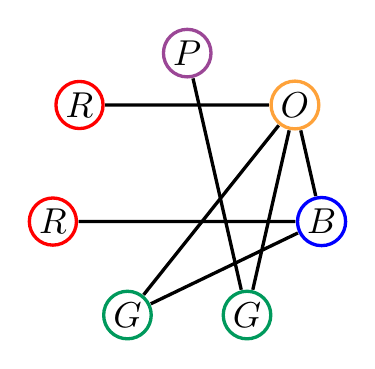
\begin{tikzpicture}[
mynode/.style={draw, circle, very thick, inner sep=1pt, scale=1.3},
myline/.style={draw, very thick},
]
\pgfmathsetmacro{\n}{7};
\pgfmathsetmacro{\r}{1.75};
\node[mynode,draw=P] (1) at (0*360/\n + 90: \r cm) {$\xcolor{P}$};
\node[mynode,draw=R] (2) at (1*360/\n + 90: \r cm) {$\xcolor{R}$};
\node[mynode,draw=R] (3) at (2*360/\n + 90: \r cm) {$\xcolor{R}$};
\node[mynode,draw=G] (4) at (3*360/\n + 90: \r cm) {$\xcolor{G}$};
\node[mynode,draw=G] (5) at (4*360/\n + 90: \r cm) {$\xcolor{G}$};
\node[mynode,draw=B] (6) at (5*360/\n + 90: \r cm) {$\xcolor{B}$};
\node[mynode,draw=O] (7) at (6*360/\n + 90: \r cm) {$\xcolor{O}$};
\draw [myline] (5) -- (1);
\draw [myline] (7) -- (2);
\draw [myline] (6) -- (3);
\draw [myline] (6) -- (4);
\draw [myline] (7) -- (4);
\draw [myline] (7) -- (5);
\draw [myline] (7) -- (6);
\end{tikzpicture}
}
\caption{\mypm{}~99563}
\end{subfigure}
%
%
%



\caption{All 12 unique graphs for \nameref{sec:ch2:example2} requiring all components to be connected and a specified number of unique edges.\label{fig:ch2:unique3}}

\end{figure*}
